\section{Entidades e Processos}

Dado o que foi discutido nos Capítulos 1 e 2 o trabalho está fundamentado no
diálogo entre a Teoria Política Espacial e a área de Dinâmicas de Opinião. Não
temos por propósito um modelo que seja preditivo, mas que capture
microfundamentos relevantes, como viés de confirmação e confiança nas crenças, e
gere distribuições de preferência plausíveis, no sentido delimitado no Capítulo
1. O trabalho propõe, portanto, um modelo que contribua para uma agenda que
busque abrir a caixa-preta do processo de socialização que leva a cristalização
de direcionamentos, ou posicionamentos, ideológicos.

Como discutido no Capítulo 1, a teoria geométrica de política modela as
preferências dos agentes como relações em um espaço contínuo de alternativas.
Essas preferências, em ambientes macro, são construídas por meio da agregação
das atitudes, crenças, posicionamentos, ou simplesmente opiniões dos agentes em
diferentes questões (\textit{issues}). As preferências dos agentes numa dimensão
são, assim, o sumário de um \textit{perfil ideológico} do agente sobre questões.
Pretendemos gerar a distribuição de pontos ideais, as posições preferidas pelos
agentes no espaço de alternativas, mas não precisamos especificar qual a função
de utilidade centrada nestes pontos, já que não é interesse do trabalho modelar
a tomada de decisão que os pressuporia, por exemplo a escolha de um candidato. É
possível atribuir diferentes funções de utilidade aos agentes, mas o pressuposto
modal é que a função vai ter um máximo e será simétrica \cite{eguia2013spatial,
  carroll2013structure}. Como não é um modelo de tomada de decisão, mas sim um
modelo de surgimento de posicionamentos ideológicos, não é necessário adicionar
mais um elemento, funções de utilidade, que simplesmente alargaria o espaço de
parâmetros e não seria utilizado na simulação. Não obstante, modelos futuros que
busquem ligar, por exemplo, a distribuição de preferências com a escolha de
candidatos/partidos poderiam fazer essa atribuição.


Pensar os agentes como tendo pontos ideais derivados de posicionamentos em
questões tem por base dois fundamentos. O primeiro é que esse elemento a mais,
em comparativo aos modelos de \citeonline{deffuant2000mixing} e de
\citeonline{martins2012bayesian}, nos permite ser mais condizentes com a
literatura discutida no Capítulo 1 em contraposição à equiparação do ponto ideal
a uma opinião. Essa equiparação passaria por cima da distinção entre crenças e
preferências \cite{list2009judgment}. Entretanto, em certos contextos, em
particular nos macro-políticos, é possível abdicar da separação estrita entre
esses dois conceitos e pensar a possibilidade de que alternativas sejam
elencadas com base em ``atitudes'' prévias
\cite{binmore2008rational,laver2014measuring}. Os pontos ideais dos
agentes vão mudar ao longo da simulação, mas isso ocorre devido à mudança nas
suas atitudes. É uma mudança assim indireta e condizente com a noção de que a
ideologia do agente é um atributo extrínseco. O segundo fundamento é que essa
modificação tem por implicação a capacidade de adicionar outros elementos à
dinâmica do modelo.

Sendo assim, cada agente na nossa população vai ter por atributo um perfil
ideológico\footnote{Nisso o modelo aproxima-se do modelo de
  \citeonline{axelrod1997dissemination}, no qual os agentes tem por atributo um
  conjunto de traços.} \(I\), onde \(I_i = (f_i(\theta_1), \ldots, f_i(\theta_n)) \). Os
elementos de \(I\) são as crenças dos agentes em cada questão. Seguindo
\citeonline{martins2012bayesian}, vamos pressupor que os agentes têm uma
probabilidade subjetiva sobre cada questão \(\theta\), um valor esperado da opinião
\( o_i = E_i[\theta]\) e incerteza \( \sigma_i^2 = E[\sigma^2] - E_ i[\theta]^2\) associados. O
ponto ideal \(x\) do agente vai ser a média aritmética ( \(x_i =
\frac{1}{n}\sum_{k=1}^{n} o_k\)) das opiniões dele em \(I\). Os pontos ideais são
implementados, portanto, como opiniões médias. Do ponto de vista da
implementação o atributo \(I\) é reduzido a um conjunto de pares \(I_i =
((o_{i,1},\sigma_{i,1}^2), \ldots, (o_{i,n}, \sigma_{i,n}^2) )\), sendo \(\sigma^2\) global, o mesmo
para todo \(i\). Logo, \(\sigma_i = \sigma\). Consideraremos também uma proporção de
agentes nos quais uma das questões tem \(\sigma\) próximo a zero\footnote{Agentes
  ``intransigentes'' ou ``inflexíveis'', discutidos mais a frente.}. Se
seguirmos \citeonline{deffuant2000mixing} e usarmos uma distribuição uniforme
(U[0,1]) para gerar os posicionamentos dos agentes na condição inicial quanto
mais vezes fizermos o sorteio dos \(o_i\) (quanto maior o número de questões),
pela Lei dos Grandes Números, mais centrada a média aritmética vai ser do valor
esperado da distribuição (0.5). Isso significa que já na condição inicial os
agentes seriam de centro. Para que isso não ocorra associamos para cada agente
uma distribuição Beta, com \(\alpha\)s e \(\beta\)s entre 1.1 e 100.

Do ponto de vista da implementação, dividimos os intervalos de valores
[1.1,100], para \(\alpha\) e \(\beta\), em \(N\) valores igualmente espaçados, onde N é o
número de agentes da população, criando uma lista do tamanho da população de
duplas \((\alpha,\beta)\). Ou seja, temos duas listas, uma com valores de \(\alpha\) entre 1.1
e 100 e outra com valores de \(\beta\) entre 1.1 e 100. Dividimos igualmente os
intervalos de acordo com o tamanho da população. Por exemplo, se a população tem
10 agentes então os valores de \(\alpha\) e \(\beta\) são [1.1, 12.0889, 23.0778,
34.0667, 45.0556, 56.0444, 67.0333, 78.0222, 89.0111, 100.0]. Misturamos as
listas para que os agentes tenham \(\alpha_i\) e \(\beta_i\) distintos, e coletamos pares
numa terceira lista. Um formato possível para essa lista é [(1.1, 56.0444),
(23.0778, 34.0667), (45.0556, 100.0), (78.0222, 67.0333), (89.0111, 23.0778),
(67.0333, 12.0889), (100.0, 78.0222), (56.0444, 1.1), (34.0667, 89.0111),
(12.0889, 45.0556)]. O primeiro agente da população vai então ter uma
distribuição Beta com parâmetros \(\alpha, \beta = (1.1, 56.0444) \), o segundo com
\(\alpha,\beta=(23.0778,34.0667)\) e assim em diante.

Destas distribuições sorteamos os valores de \(o_i\) iniciais para cada questão,
de forma que os \(o\)s de cada agente são correlacionados e as distribuições são
centradas em diferentes pontos do espaço, como ilustrado na Figura
\ref{fig:betas100}:

\begin{figure}[H]
  \centering
  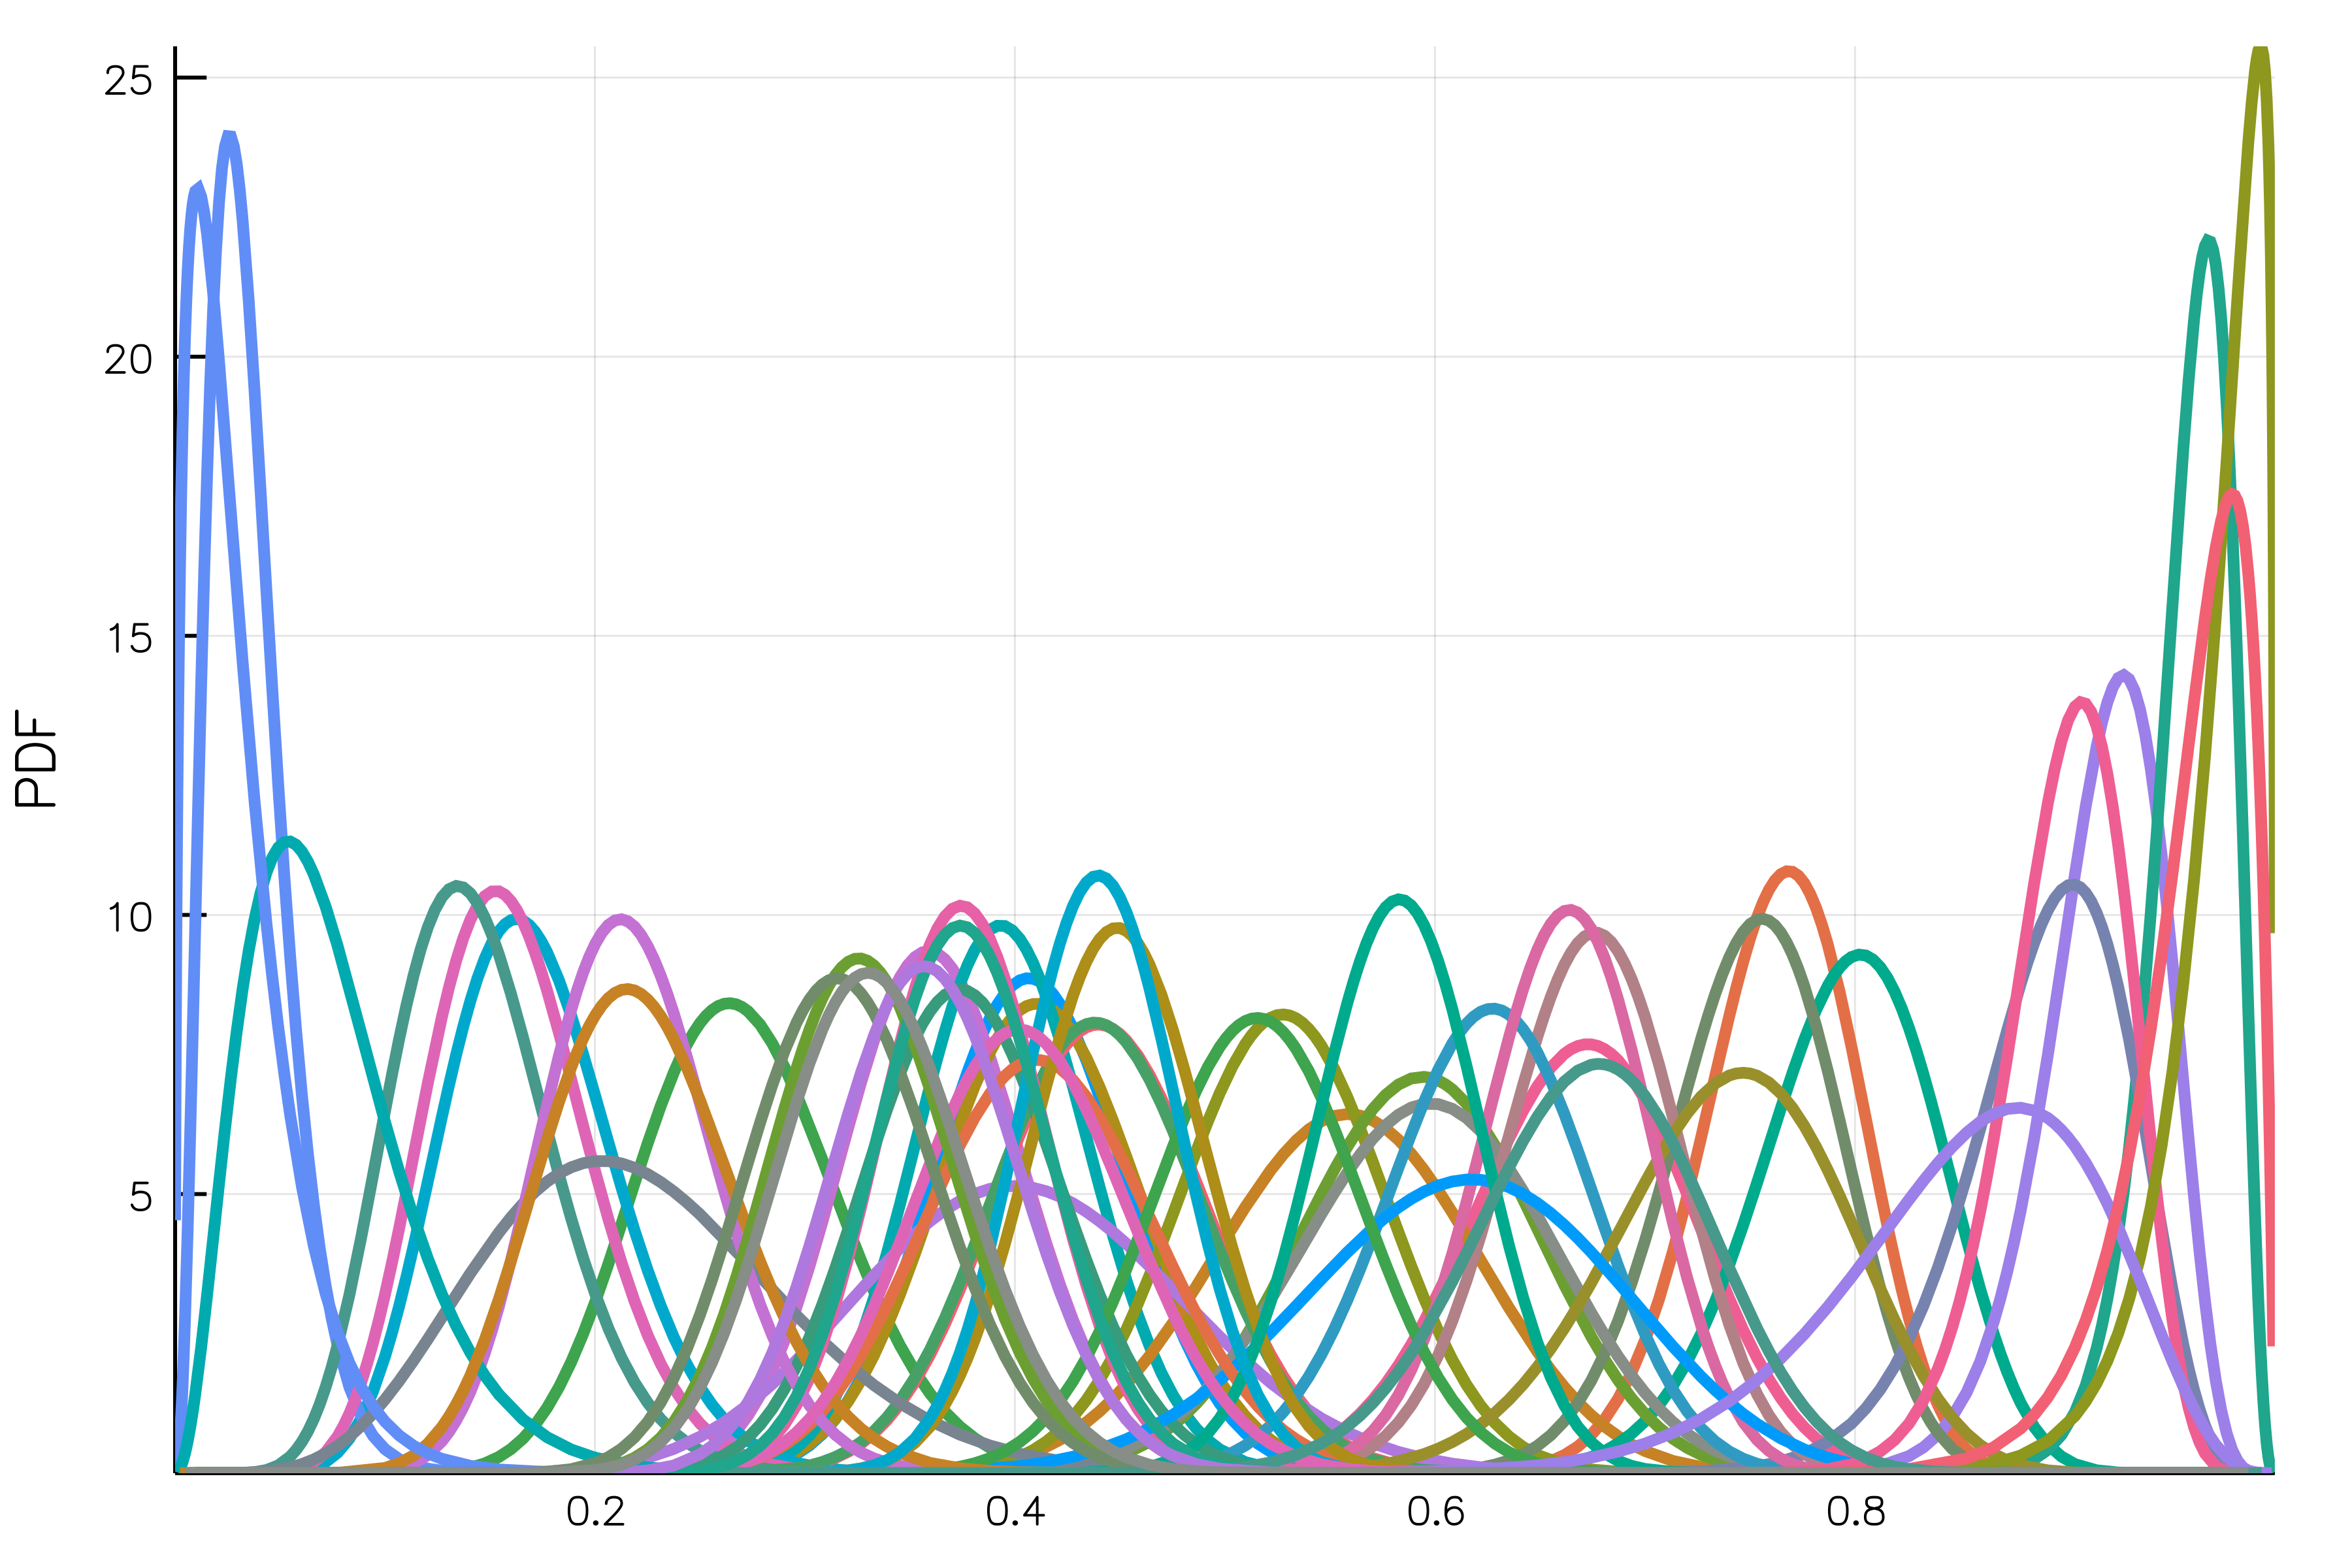
\includegraphics[width=\textwidth]{ims/beta100.png}
  \caption{Distribuições Beta para 50 agentes}
  \source{ Elaborada pelo autor.}
  \label{fig:betas100}
\end{figure}


A cada iteração da simulação um dos agentes vai ser escolhido e vai interagir
com um de seus vizinhos, a princípio num grafo completo imposto exogenamente
(estabelecemos na condição inicial quais os vizinhos). Quanto à implementação,
criamos um grafo de tamanho igual ao tamanho da população e fazemos com que cada
agente da população tenha como um de seus atributos um conjunto de vizinhos
igual a um vértice do grafo. A interação é em díades, assíncrona (os
agentes atualizam seus atributos em momentos distintos) e sequencial (um agente
atualiza por vez) \cite{wilensky2015introduction}. A dependência dos resultados
em relação ao número de agentes e de crenças vai ser explorada. Estamos
interessados nas alterações ao longo prazo (em termos de iterações) da
configuração dos \(x\) sob diferentes combinações de parâmetros, tendo em vista
as interações dos agentes \cite{acemoglu2011opinion} \footnote{Como vamos
  definir longo prazo e analisar o modelo é tema da seção metodológica.}.

Quando os agentes interagem o agente \(i\) atualiza sua opinião em
alguma\footnote{ Uma outra implicação possível, a ser adicionada em trabalhos
  futuros, é considerar um viés nessa seleção, o que representaria saliência no
  sentido dado por \citeonline{zaller1992simple}: qual questão os agentes estão
  dando atenção, qual questão está mais acessível na memória deles.} questão
segundo as equações 2.3 e 2.4. Qual questão vão ``debater'' vai ser definido por
meio de um sorteio sem viés. Se o agente tem uma lista indexada \(l\) de
opiniões sorteamos um índice que determina qual a questão de debate, por meio de
um sorteio onde cada índice tem igual probabilidade de ser selecionado. Dado que
os agentes agora tem um conjunto de opiniões é plausível considerar que um
conjunto de agentes tenham determinadas opiniões em que eles tenham maior
certeza, identificação, ou centralidade para o seu perfil ideológico. Sendo
assim na condição inicial alguma proporção de agentes tem uma questão no seu
perfil \(I\) cujos \(\sigma\) associados são aproximadamente zero. Com isso buscamos
analisar o papel de agentes ``inflexíveis'' na dinâmica populacional. A
proporção de agentes intransigentes ou inflexíveis é assim um parâmetro da
simulação.

Os agentes também vão reconsiderar suas opiniões e certezas sobre as questões
segundo um ruído. Do ponto de vista teórico, estamos considerando a
possibilidade de fatores não relacionados à influência social levarem o agente a
mudar seu posicionamento sobre questões \cite{flache2017, lorenz2017modeling}.
Do ponto de vista metodológico, \citeonline{macy2015signal} argumenta que
pequenas perturbações no comportamento local dos agentes podem levar a mudanças
drásticas nas propriedades sistêmicas. Particularmente, consideram que adicionar
ruído pode: eliminar equilíbrios frágeis, o que reduz o conjunto de resultados e
tornando-os mais previsíveis; e embora aumente a heterogeneidade local isso pode
acabar facilitando interações sociais que reduzem a diversidade global
\cite[p.323]{macy2015signal}. A nova opinião \(o(t+1)\) é igual a \(o(t) + r\),
onde \(r\) é retirado de uma distribuição normal de média 0 e desvio padrão
\(\rho\), um parâmetro da simulação. No caso em que o agente seja
intransigente na questão ele não será sujeito ao efeito do ruído \footnote{Uma
  outra opção seria que agentes intransigentes sejam \textit{menos} afetados
  pelo ruído. Optamos pela mais simples.}


\section{Parâmetros-Chave}

Os parâmetros-chave para configuração e inicialização do modelo, cujos valores
seguem \citeonline{martins2008continuous}, \citeonline{deffuant2000mixing} e
\citeonline{lorenz2017modeling}, são:

\begin{itemize}
\item A população de \(500 < N < 5000\) agentes;
\item O número de questões \(1 \leq \text{n\_issues} \leq 10\); 

\item As incertezas \(0.01 \leq \sigma_i \leq 0.5\);
  \begin{itemize}
  \item Agentes intransigentes vão ter uma de suas opiniões com incerteza
    próxima a zero (\(1e-20\));
  \end{itemize}

\item O parâmetro de confiança \(0.1 \leq p \leq 0.99\);
  
\item A proporção de agentes intransigentes \(0.0 \leq (\text{p\_intran}) \leq 0.1\);

\item O parâmetro de reconsideração \(0.0 < \rho  \leq 0.1\), onde \(\rho\) é o desvio
  padrão de uma Normal de média 0:
  \begin{itemize}
  \item Isso significa que o ruído, \textit{r}, é sorteado a partir de uma
    normal N(0,\(\rho\)), de forma que \(o(t+1) = o(t) + r\);

    \begin{itemize}
    \item Se \(o(t) + r > 1\) então \(o(t+1) = 1\);
    \item Se \(o(t) + r < 0\) então \(o(t+1) = 0\).
    \end{itemize}
    
  \end{itemize}
 
\end{itemize}

\section{Inicialização e Iteração}

A inicialização da simulação depende dos parâmetros-chave apresentados. Na
condição inicial temos uma população de \(N\) agentes, que tem por atributos: um
conjunto de pares \(I_i = ((o_{i,1},\sigma_{i,1}^2), \ldots, (o_{i,n},\sigma_{i,n}^2))\), onde
o número de questões, \(n\), é uma variável global, cada \(o\) é retirado de uma
distribuição Beta(\(\alpha,\beta\)), onde cada agente tem um \(\alpha\) e um \(\beta\) próprio,
com valores\footnote{Paramêtros com valores \(\leq\) 1 ou geram distribuições de
  formato uniforme, quando \(\alpha = \beta = 1.0\), ou com formato de U. Quanto ao
  limiar superior, o valor de 100 permite que tenhamos agentes com distribuições
  centralizadas em ambos os extremos, dado que a média \(\mu\) é dada por
  \(\frac{\alpha}{\alpha + \beta}\), de forma que a média mínima é 0.011.} entre 1.1 e 100.

Voltando aos atributos dos agentes, o\(\sigma^2\) é uma variável global de forma que
\(\sigma_i^2 = \sigma^2\) ; têm também por atributo um posicionamento ideológico, ou ponto
ideal, \(x_i = \frac{1}{n} \sum_{k = 1}^n o_{i,k} \); e um conjunto de vizinhos, o
qual depende de qual a rede os agentes estão. Uma determinada proporção de
agentes vai ter um \textit{único} \(\sigma_i = (1e-20 ) \approx 0.0 \). Quantos agentes são
intransigentes em \textit{uma} questão é dado por \(\text{p\_intran}\). Em qual
questão vão ser intransigentes é aleatório, sorteado de seu \(I\).

Uma iteração da simulação, a passagem de \(t\) para \(t+1\), é dada pela
aplicação de dois procedimentos: a atualização da opinião via influência social
e a atualização aleatória. Uma repetição da simulação é a aplicação iterativa
desses dois procedimentos ao longo de um tempo \(t \). O procedimento de
influência social é o seguinte: sorteamos um agente \(i\) da população. Então
sorteamos um de seus vizinhos, o agente \(j\). Sorteamos uma das questões \(k \in
(1,\ldots,n)\) de forma que temos os \((o_{i,k},o_{j,k})\) e
\((\sigma_{i,k}^2,\sigma_{j,k}^2)\) correspondentes à questão. Então o agente \(i\)
atualiza \(o_{i,k}\) segundo as equações 2.3 e 2.4. Essa regra é um parâmetro
global da simulação, o que significa que a cada repetição todos os agentes
atualizam suas crenças segundo a mesma regra. Ademais, temos o ruído. A cada
iteração temos os efeito da influência social \textit{e} do ruído. Novamente
escolhemos um agente da população. Sorteamos uma questão de forma que temos
\(o\) e \(\sigma^2\) correspondentes. Se o agente é intransigente naquela questão
então ele não muda de opinião. Sorteamos um \(r\) retirado de uma distribuição
normal \(N(0,\rho)\) e atualizamos \(o\) de forma que \(o(t+1) = o(t) + r\). Os
\(x_i\), o objeto de interesse de análise, são atualizados sempre que ocorrerem
mudanças nas crenças dos agentes.

\section{Metodologia de Análise}

Dentre as diversas formas de analisar um ABM a análise de sensibilidade global
se destaca como uma forma de ter uma compreensão ampla, geral, do comportamento
do modelo \cite{north2007managing}. O primeiro passo da análise envolve, então,
 ter uma compreensão geral do comportamento do modelo para então passarmos
para regiões particulares do espaço de parâmetros.

No entanto, o alto custo computacional de varrer esse espaço de parâmetros faz com
que só seja possível realizarmos uma análise global, na maioria dos casos, se
seguirmos métodos formais da literatura de análise de sensibilidade
\cite{railsback2012agent}. Esses métodos trazem o benefício de determinar como
selecionar subconjuntos de todas as combinações de parâmetros, reduzindo o
número de realizações necessárias da simulação e de trazerem formas sistemáticas
de interpretar os resultados \cite{railsback2012agent}.


\begin{figure}[h]
    \centering
    \begin{subfigure}[b]{0.49\textwidth}
      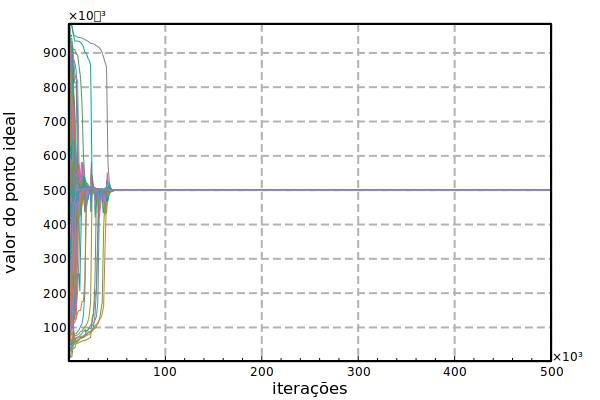
\includegraphics[width=\textwidth]{ims/timeseries1.png}
      \caption{\( \sigma = 0.1\) }
    \end{subfigure}
    \begin{subfigure}[b]{0.49\textwidth}
      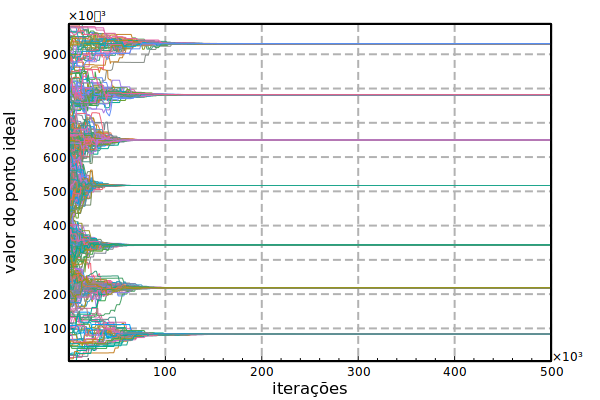
\includegraphics[width=\textwidth]{ims/timeseries2.png}
       \caption{\(\sigma = 0.02\) }
      \end{subfigure}
      \caption{Evolução dos pontos ideais dos agentes ao longo de duas realizações.
        Parametrização: \(  N = 500, p = 0.9, \rho =  1e-5, n\_issues = 1 , p\_intra
        n= 0.0 \)}
      \source{ Elaborada pelo autor.}
      \label{fig:tseries1}
    \end{figure}
    
    Antes de discutirmos métodos de amostragem e análise, é necessário
    estabelecer uma medida do sistema para que possamos analisá-lo
    \cite{railsback2012agent}. Escolhemos o desvio padrão dos pontos ideais após
    \(1.000.000\) iterações como output para análise\footnote{Testamos diversas
      parametrizações com n\_issues \(= 1\) e observamos que a partir de
      \(50.000\) iterações a implementação replica os resultados de
      \citeonline{martins2009bayesian}.}, dado que nos diz o quão
    concentrados/dispersos são os pontos ideais da população. Uma outra opção de
    medida do sistema seria o número de opiniões finais distintas após as
    iterações, o que nos daria uma medida de ``cobertura'' do sistema: uma maior
    cobertura equivale a um número maior de posicionamentos distintos
    \cite{bramson2016disambiguation}. Na \ref{fig:coverage} a distribuição (b)
    tem maior cobertura dado que uma maior quantidade de espaço é preenchido.
    
    \begin{figure}[H]
      \centering
      \includegraphics[width =12cm]{ims/coverage.png}
      \caption{Distribuições com coberturas distintas}
      \source{\citeonline{bramson2016disambiguation}}
      \label{fig:coverage}
    \end{figure}

    
    Usar cobertura como medida não nos indica
    o quão diferente são os valores, ou se estão no centro ou extremos, mas
    captura a variedade de atributos \cite[p.85]{bramson2016disambiguation}.
    Contudo, teríamos que estabelecer um \(N\) base, pois de outra forma esse
    parâmetro explica quase que totalmente o valor do output a ser analisado
    pela análise de sensibilidade.
    
    No primeiro gráfico da figura \ref{fig:tseries1} temos um desvio padrão
    próximo zero, e um único posicionamento ideológico final. Já no segundo
    gráfico precisaríamos arredondar os pontos ideais finais, para entre 1 e 6
    casas decimais, para chegarmos a conclusão que existem cerca de 6 pontos de
    convergência. Se não arredondarmos o resultado final teríamos uma medida
    próxima de 500 pontos ideais, e que não nos informaria a respeito da
    cobertura do sistema. Já o desvio padrão nos indica a dispersão dos pontos
    ideais, pois tem valor de aproximadamente 0.24, próximo ao da condição
    inicial. Um outro problema do uso do número final de pontos ideais ao fim de
    uma realização é que a medida não é robusta a ruídos ou proporções de
    agentes intransigentes diferentes de 0. Quando há ruído ou agentes
    intransigentes o número final de pontos ideais não informa muito sobre a
    dinâmica do sistema. Na Figura \ref{fig:nonnullrho} temos um comportamento
    qualitativamente similar ao da Figura \ref{fig:tseries1} (b), do ponto de
    qualitativo seriam 6 opiniões médias com oscilações ao redor delas, mas
    quantitativamente o número de opiniões finais distintas é próximo de 500.
    Uma opção para tentar capturar em medidas essa oscilação ao redor de 6
    opiniões médias seria medirmos o número de pontos ideais finais com valores
    arredondados. Arredondar demais faz com que perdamos a comparabilidade com a
    condição inicial, que passa a não ter mais 500 pontos ideais. No caso da
    figura \ref{fig:nonnullrho} usar o número de pontos ideais distintos como
    medida nos informa que há grande cobertura no sistema, mas passaria
    despercebido o fato de que ao fim o comportamento é bastante similar ao caso
    com ruído nulo. O desvio padrão não nos informa sobre a existência dos
    ``clusters'', mas ao menos mantêm a consistência nos casos com e sem ruído.
    
  \begin{figure}[H]
    \centering
    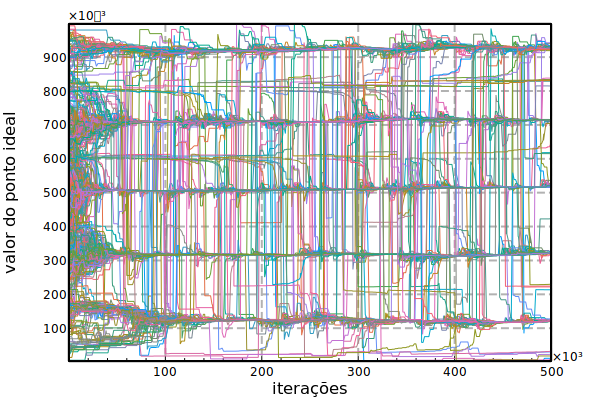
\includegraphics[width =10cm]{ims/ts5.png}
    \caption{Parametrização equivalente a Figura \ref{fig:tseries1} (b),
      mas com \(\rho = 0.001\).}
    \source{ Elaborada pelo autor.}
    \label{fig:nonnullrho}
  \end{figure}

Quanto à amostragem uma estratégia comum são as parametrizações de Monte Carlo:
sortear valores de parâmetros usados para as realizações das simulações a partir
de distribuições uniformes nos intervalos de valores dos parâmetros
\cite{laver2011party}. O problema dessa estratégia é que o espaço de parâmetros
não é coberto igualmente, havendo a possibilidade de pontos de acumulação ou
espaços vazios \cite{pereda2017brief}.

\citeonline{saltelli2008global} argumenta que para manter uma dispersão
equitativa dos pontos no espaço de parâmetros é necessário um algoritmo que
enviese a seleção de novos pontos para mantê-los afastados dos pontos já
presentes. O pacote de Python SaLib\footnote{Fazemos uso da interoperabilidade
  entre a linguagem Julia e Python, por meio do pacocte PyCall
  \cite{johnson2018}.}, o qual usamos, implementa ``samplers'' que garantem essa
dispersão equitativa por meio da geração de amostras sorteadas de sequências
quasi-aleatórias de baixa discrepância \cite{herman2017salib}. \footnote{ Se
  pensarmos os parâmetros geometricamente podemos pensar num ``espaço'' de
  parâmetros que queremos preencher de maneira equitativa. A discrepância de uma
  sequência de pontos é a diferença absoluta máxima de um conjunto de regiões,
  no espaço de parâmetros, entre a fração de pontos e a fração de área. Por
  exemplo, se tivermos um quadrado unitário com 20 pontos, e o dividirmos em 16
  quadrados menores de tamanho \(\frac{1}{6}\) e distribuirmos os pontos de
  forma equitativa os quadrados deveriam ter 1 ou 2 pontos. Se um dos quadrados
  tiver 5 pontos, contudo, a discrepância será de ao menos \(\frac{5}{20} -
  \frac{1}{16} = \frac{3}{16}\) \cite[p.83]{saltelli2008global}. Para a
  implementação do ``sampler'' ver
  \url{http://salib.readthedocs.io/en/latest/_modules/SALib/sample/saltelli.html}.}

O tamanho amostral e número de parametrizações não independe do método de
análise, dado que incorrem em custos computacionais distintos
\cite{saltelli2002making}. Seguimos \citeonline{jaxa2018pynetlogo} e
\citeonline{brookes2015saltelli} em usar o esquema de
\citeonline{saltelli2002making} para o cálculo de índices de sensibilidade
global. Fazendo uso de sequências quasi-aleatórias, ele consiste em gerar n *
(2d + 2) parametrizações, onde \(n\) é o tamanho amostral  e \(d\) é o
número de parâmetros. Segundo \citeonline[p.284]{saltelli2002making} esse número
de parametrizações nos permite calcular índices de Sobol de primeira e segunda
ordem e índices totais, discutidos no parágrafo seguinte. No nosso caso \(d =
6\), pois vamos ter como parâmetros : N (população), número de questões
(codificado como n\_issues ), \(p\), \(\sigma\), a proporção de agentes
intransigentes (codificado como p\_intran), e \(\rho\). Quanto maior o tamanho da
amostra  menor os coeficientes de erro para os índices. Para garantir um
coeficiente de erro baixo no cálculo subsequente dos índices de sensibilidade
especificamos um tamanho amostral base \(n\) de \(5000\), de forma que rodamos
\(70.000\) parametrizações. Nos limitamos a esse número de parametrizações pelo
custo computacional de simular tantas parametrizações : aproximadamente 60 horas
\footnote{Numa máquina: Intel(R) Core(TM) i7-6500U CPU @ 2.50GHz, com 15.4GiB de
  RAM.}. Os baixos valores dos coeficientes de erro nos confirmam que amostras
maiores não seriam necessárias.

%\todo[inline,color = yellow!10]{Comentário: A discussão precisa sobre a relação entre
%  indices e número de avaliações esta em \citeonline{saltelli2002making}, e
%  envolve método de monte carlo. Sinceramente, não tenho o treinamento matemático
%  para esmiuçar essa questão... faço uso do método para dar \textit{algum} rigor
%metodológico ao trabalho, para que as escolhas metodológicas não sejam
%arbritárias. Sei que poderia ser melhor explicado, mas só compreendo por cima e
%conceitualmente...}

Para a análise, seguimos \citeonline{ten2016sensitivity} e combinamos
histogramas da medida do sistema, gráficos de dispersão e índices de
sensibilidade. Os índices de sensibilidade utilizados são os índices de Sobol,
particularmente índices de Sobol de primeira ordem e totais
\cite{saltelli2008global}. Os índices de Sobol decompõem o impacto dos
parâmetros na variância do \textit{output} de interesse. Os índices de primeira
ordem incluem contribuições lineares e não-lineares dos parâmetros, mas não
efeitos interativos \cite{ten2016sensitivity}. Dois fatores interagem quando o
seu efeito conjunto sobre o output não pode ser expresso como a soma de seus
efeitos individuais\footnote{Essa é a definição usual de efeito interativo no
  contexto da análise multivariada de dados \cite{hair2009analise}.}. Já índices
totais incluem todos os efeitos de ordem maior decorrentes das interações entre
os parâmetros. Digamos que temos um modelo com 3 fatores. O efeito total,
\(S_{T1}\) do primeiro fator \(X_1\) é dado pela soma dos termos da equação
\(S_{T1} = S_1 + S_{12} + S_{13} + S_{123}\), onde \(S_i =
\frac{V[E(Y|X_i)]}{V(Y)}\), \(S_{12}\) é o impacto na variância de \(Y\), o
output, da interação entre \(X_1\) e \(X_2\), sendo portanto o efeito conjunto
de \(X_1\) e \(X_2\) menos os efeitos de primeira ordem para esses fatores:
\(S_{ij}\) = \(\frac{V[E(Y|X_i,X_,)] - V[E(Y|X_i)] - V[E(Y|X_j)]}{V(Y)} \); a
mesma lógica é aplicada aos outros termos \footnote{ Para maiores detalhes do
  cálculo dos índices ver \citeonline[p.159-167]{saltelli2008global}.}. O índice
total informa características não aditivas de um modelo, de forma que para um
fator \(X_j\) uma diferença significativa entre \(S_{Tj}\), seu efeito total, e
\(S_j\), seu efeito individual, aponta para um efeito interativo desse fator com
outros fatores. Num modelo puramente aditivo a soma dos índices de primeira
ordem \(\sum_{i=1}^k S_i\) é igual a 1, isto é, nesse caso o output seria
totalmente explicado pela soma dos efeitos individuais
\cite{saltelli2008global}. Num modelo em que \(S_i = 1\) e todos os outros
\(S_{ij} = 0\) teríamos um modelo explicado por um único fator. Se \(S_1 = 0\)
então esse fator não explica nada a variância do output. O usual, contudo, é que
o modelo seja explicado parcialmente por certos fatores, e parcialmente pela
interação deles.


\section{Resultados}

Rodamos então \(70.000\) parametrizações por \(1.000.000\) de iterações tendo
por \(Y\), o \textit{output} de interesse, o desvio padrão  dos pontos ideais da
população (\(\text{Ystd}\)) após as iterações. São \(6\) os parâmetros de input
: o número de agentes (\(N\)), o número de questões (\(\text{n\_issues}\)), o
parâmetro de confiança (\(p\)), a incerteza (\(\sigma\)),  o ruído \(\rho\), e a
proporção de agentes intransigentes (\(p\_intran\)) nos
limiares apresentados na seção Parâmetros-Chave.

Como uma primeira aproximação do comportamento geral do modelo, a Figura
\ref{fig:hists1} apresenta a dispersão dos pontos ideais na condição inicial e
ao fim das simulações para cada parametrização.

\begin{figure}[h]
    \centering
    \begin{subfigure}[b]{0.49\textwidth}
      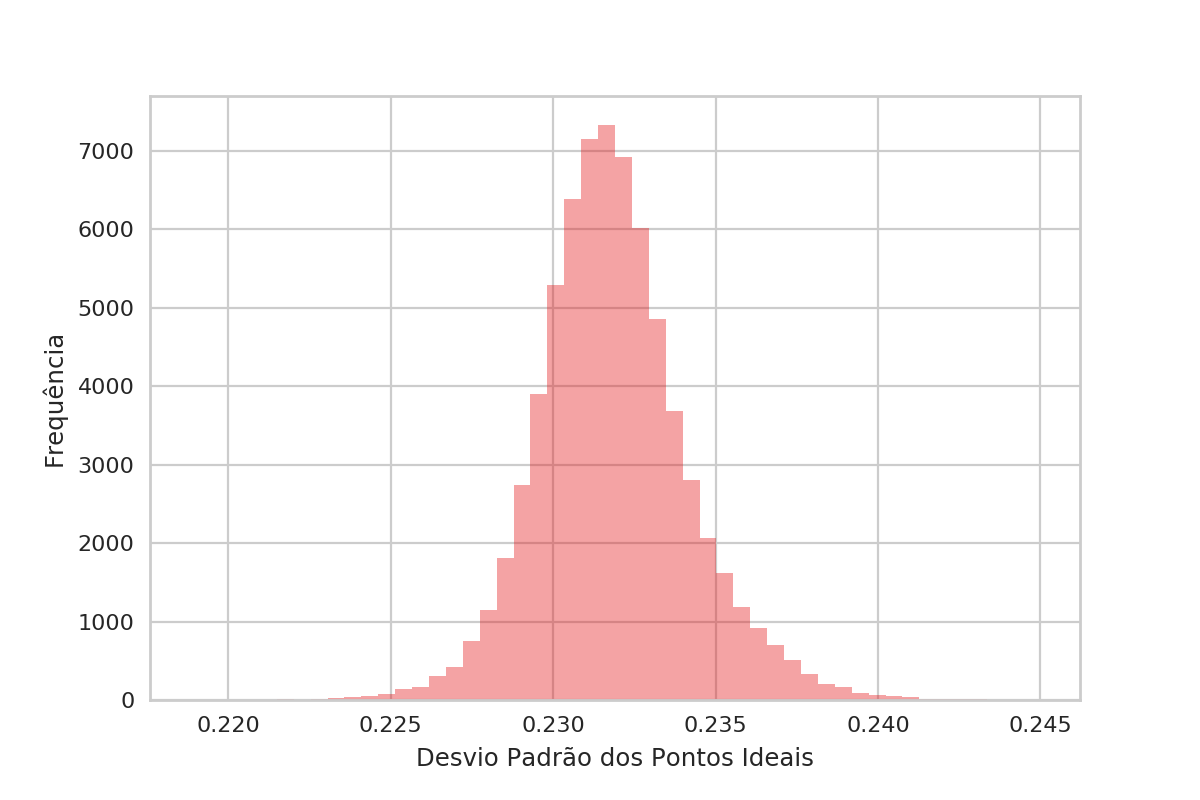
\includegraphics[width=\textwidth]{ims/diststdinit.png}
      \caption{Condição inicial}
    \end{subfigure}
    \begin{subfigure}[b]{0.49\textwidth}
      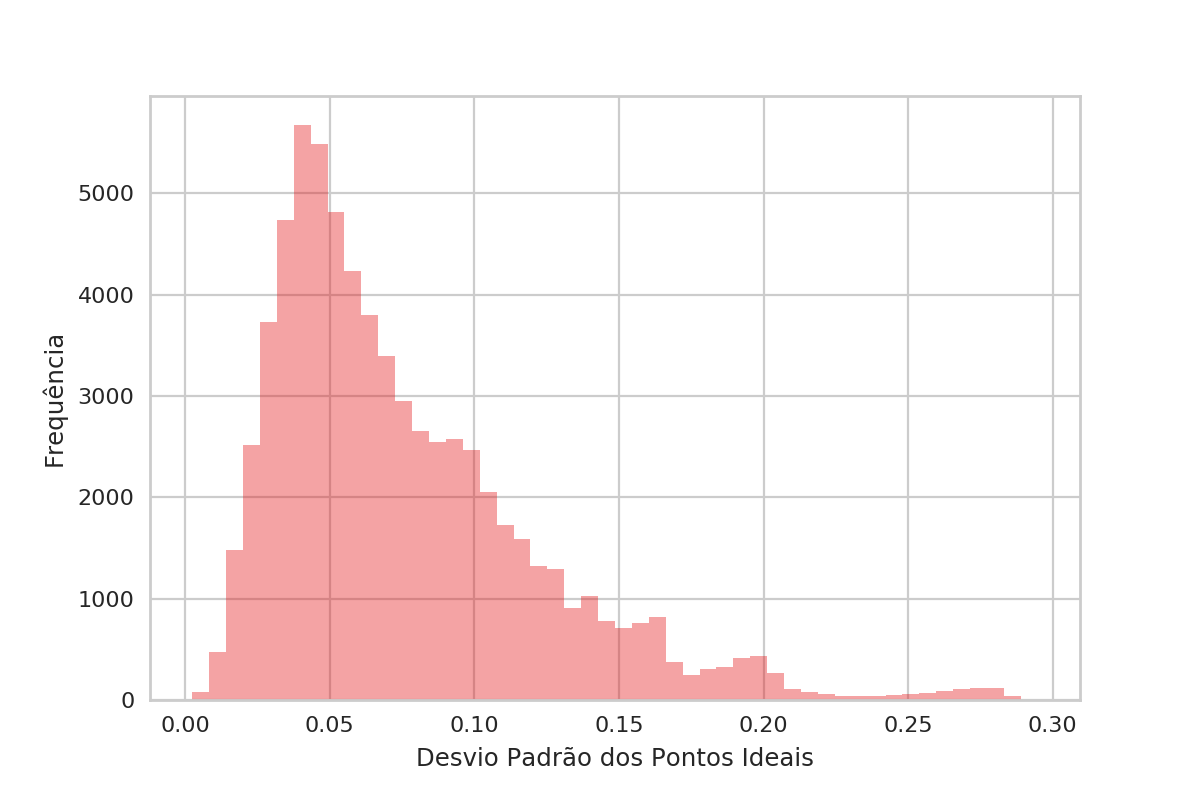
\includegraphics[width=\textwidth]{ims/distY.png}
       \caption{Após 1.000.000 iterações}
      \end{subfigure}
      \caption{Desvio padrão dos pontos ideais das populações para cada
        parametrização}
      \source{ Elaborada pelo autor.}
      \label{fig:hists1}
    \end{figure}
    
%
%
%\begin{figure}[H]
%  \centering
%  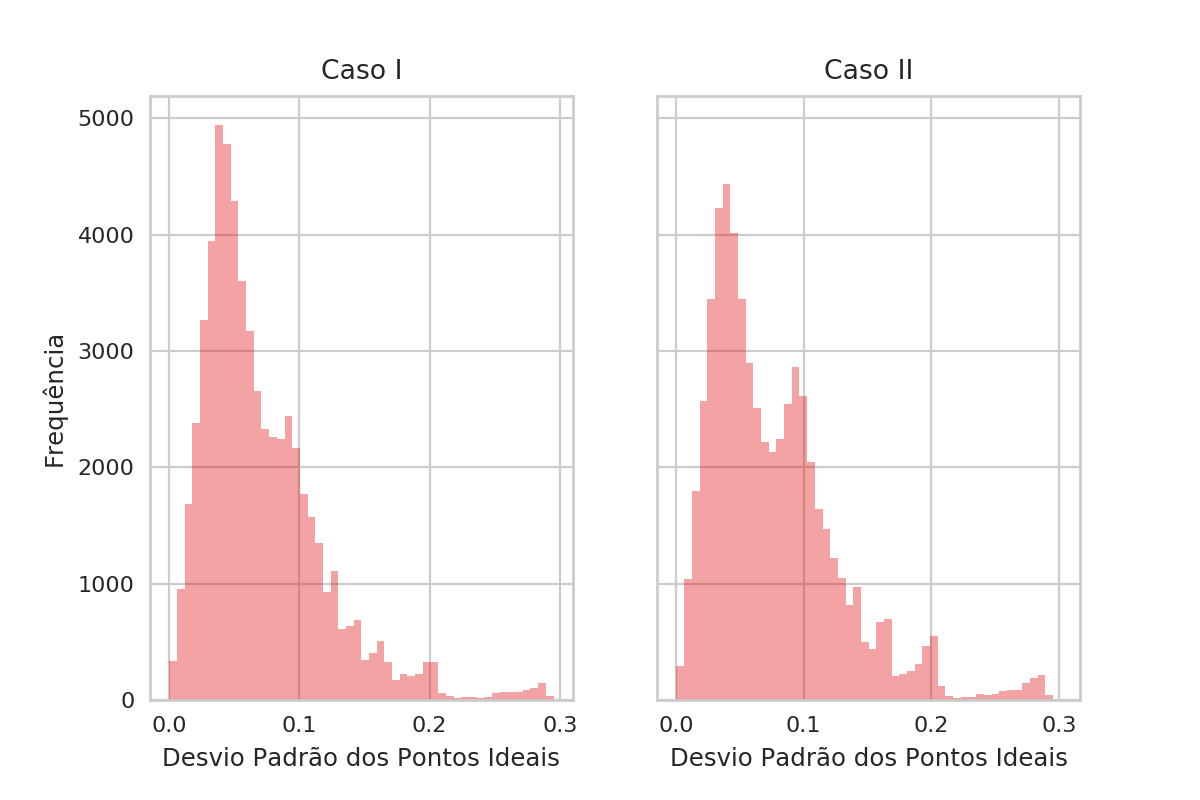
\includegraphics{ims/distYs.png}
%  \caption{Output (desvio padrão dos pontos ideais) }
%  \label{fig:Yshist}
%\end{figure}

    A Figura \ref{fig:hists1} nos leva a interpretar que a aplicação iterativa
    do procedimento do modelo, deixa a distribuição de opiniões menos dispersa,
    com uma maior concentração das parametrizações em outputs de baixa dispersão
    (entre 0.0 e 0.1). Isso condiz com as regras de atualização (assimilativa,
    mas na qual agentes distantes tem pouco impacto na opinião um dos outros) e
    com o fato dos agentes terem por vizinhos todos os outros agentes. Os
    agentes ao interagirem ou ficam mais parecidos ou não são influenciados. O
    modelo tem assim uma forte tendência assimilativa, ao menos num grafo
    completo. Todavia, a figura não nos informa qual parâmetro é responsável por
    isso, ou quais os valores de concentração (centrais ou extremos).

    A primeira pergunta pode começar a ser respondida por meio de gráficos de
    dispersão. A partir da Figura \ref{fig:scatter1} podemos inferir que há uma
    relação negativa entre os parâmetros \(\text{n\_issues}, p, \sigma \) e a
    dispersão dos pontos ideais (\( \text{Ystd}) \). A relação entre \(p\) e
    \(\sigma\) são explicadas pelo fato de agentes que ``confiam'' mais na opinião
    dos outros agentes e são mais incertos vão convergir mais rápido para a
    mesma opinião.

\begin{figure}[H]
    \centering
    \begin{subfigure}[b]{0.49\textwidth}
        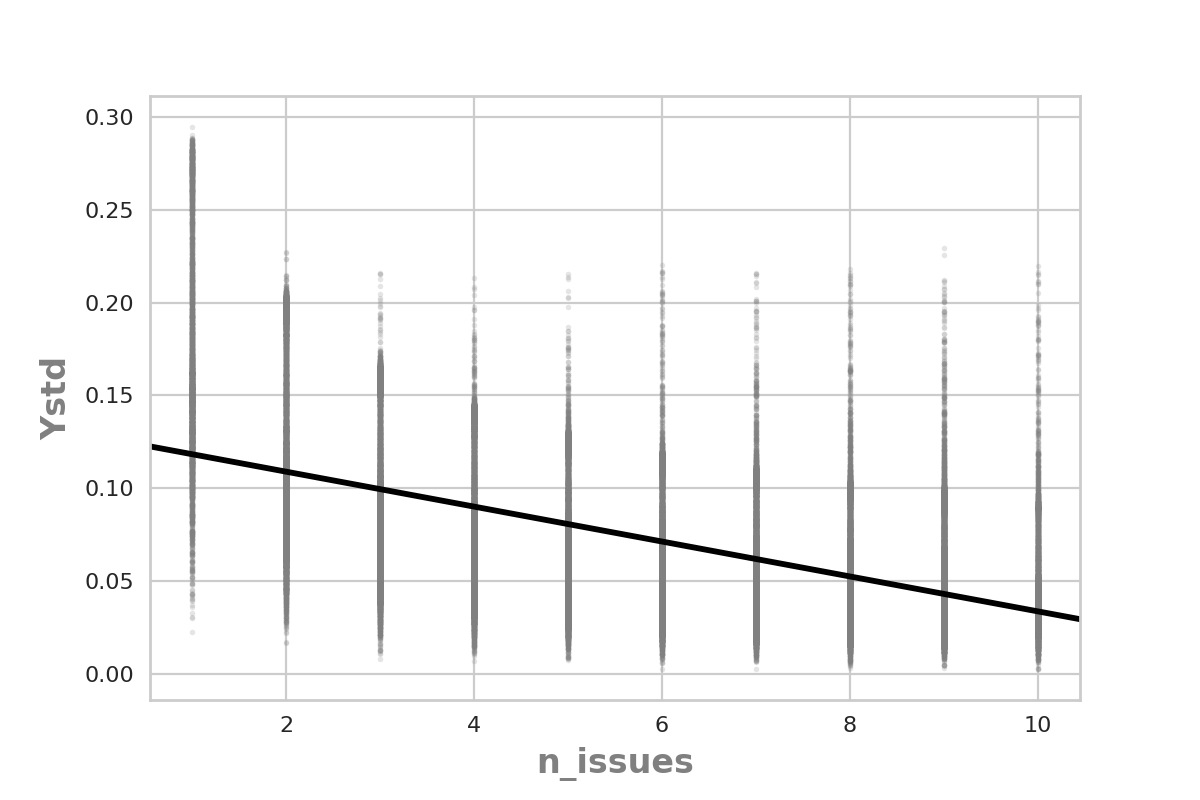
\includegraphics[width=\textwidth]{ims/mutoregressions/regressionmutatingon_issues.png}
    \end{subfigure}
    \begin{subfigure}[b]{0.49\textwidth}
        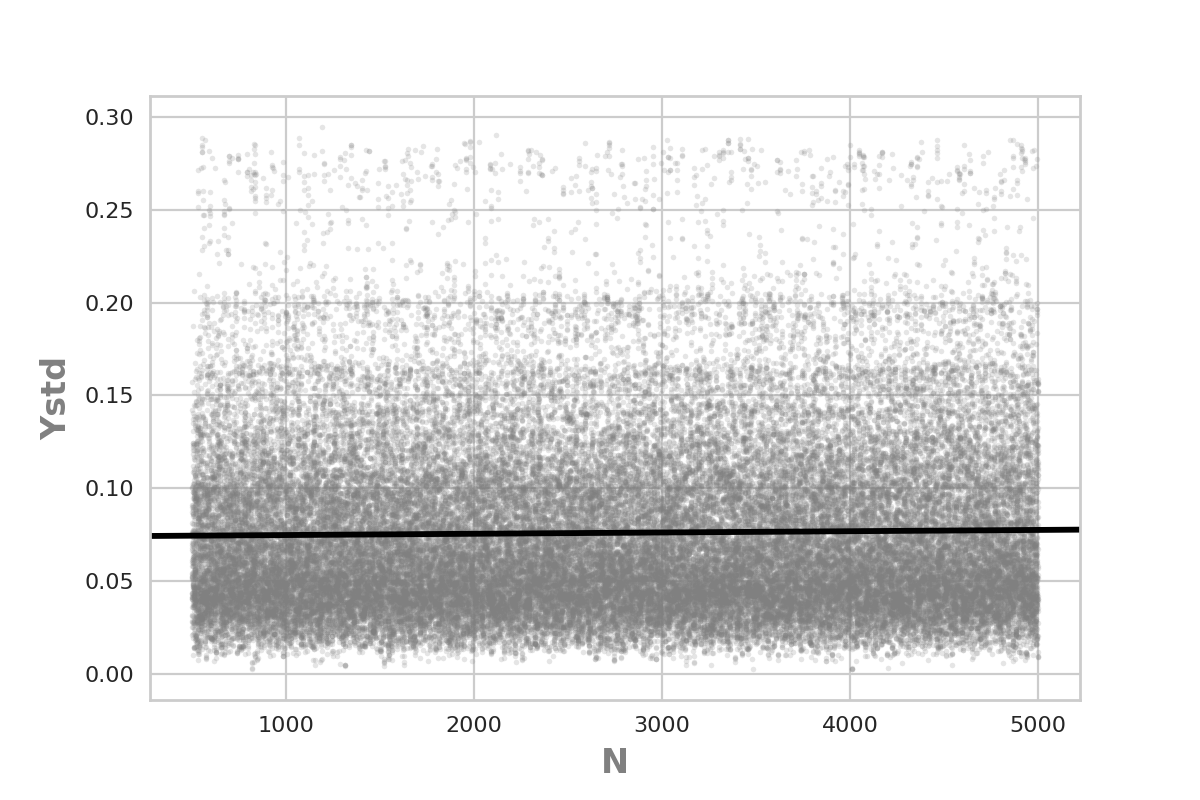
\includegraphics[width=\textwidth]{ims/mutoregressions/regressionmutatingoN.png}
    \end{subfigure}

    \begin{subfigure}[b]{0.49\textwidth}
        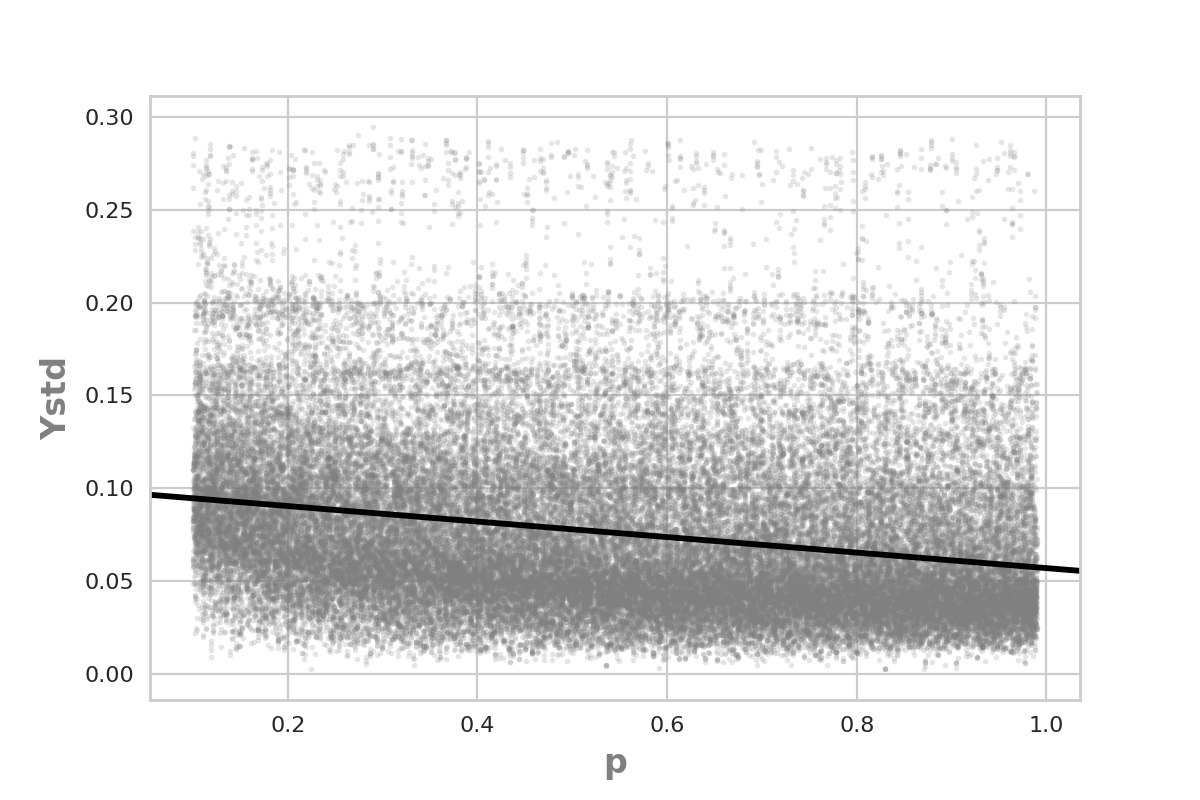
\includegraphics[width=\textwidth]{ims/mutoregressions/regressionmutatingop.png}
      \end{subfigure}
          \begin{subfigure}[b]{0.49\textwidth}
            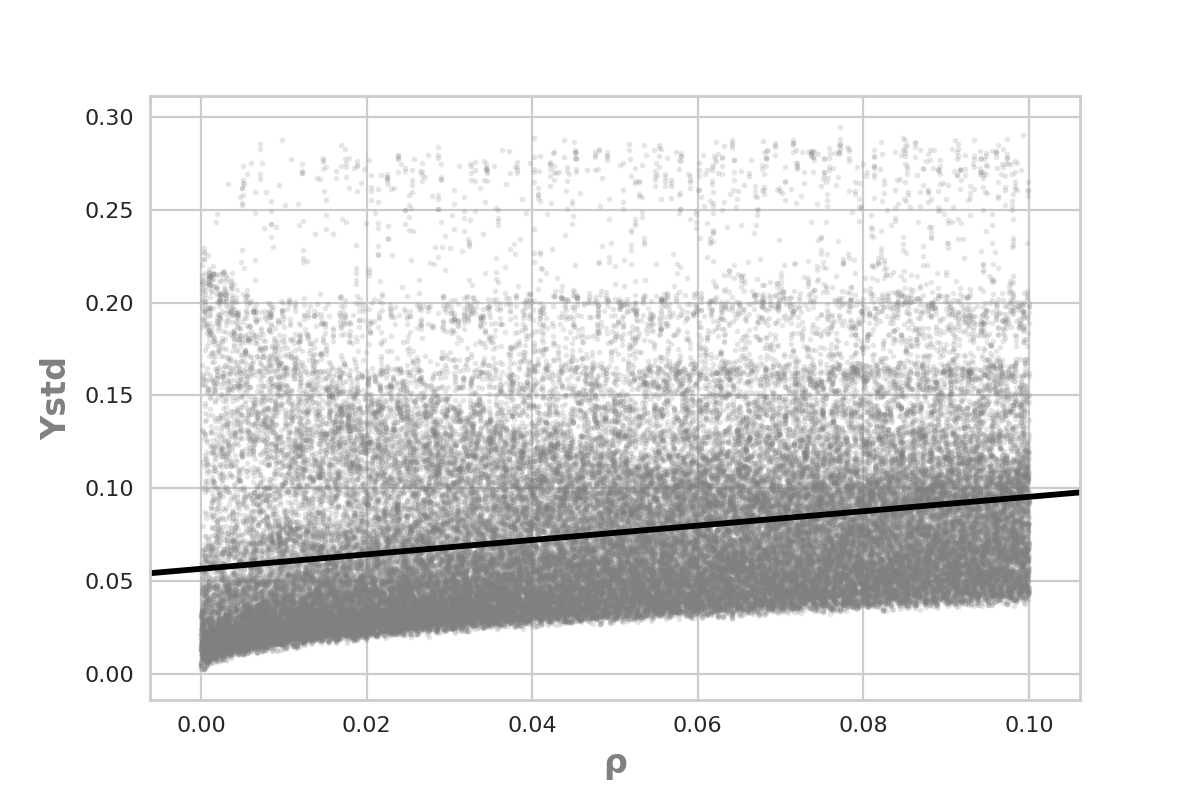
\includegraphics[width=\textwidth]{ims/mutoregressions/regressionmutatingorho.png}
      \end{subfigure}

                \begin{subfigure}[b]{0.49\textwidth}
            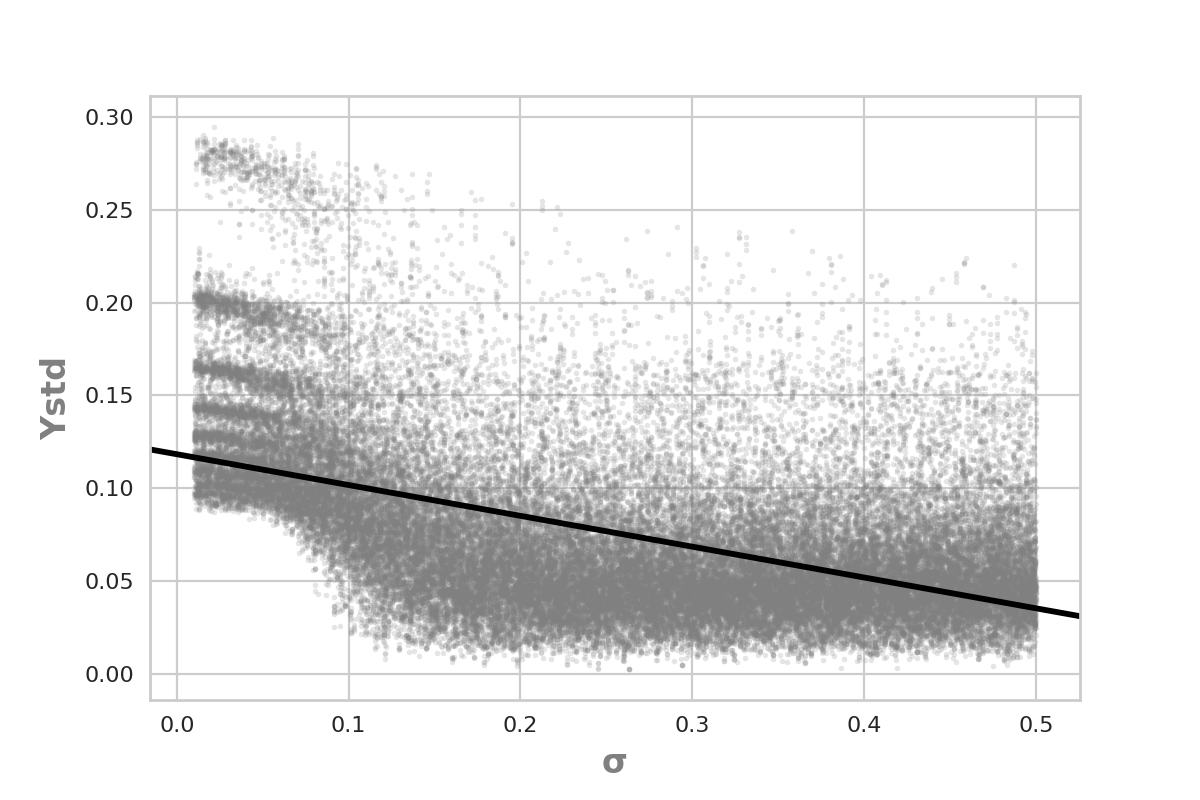
\includegraphics[width=\textwidth]{ims/mutoregressions/regressionmutatingosigma.png}
          \end{subfigure}
                \begin{subfigure}[b]{0.49\textwidth}
            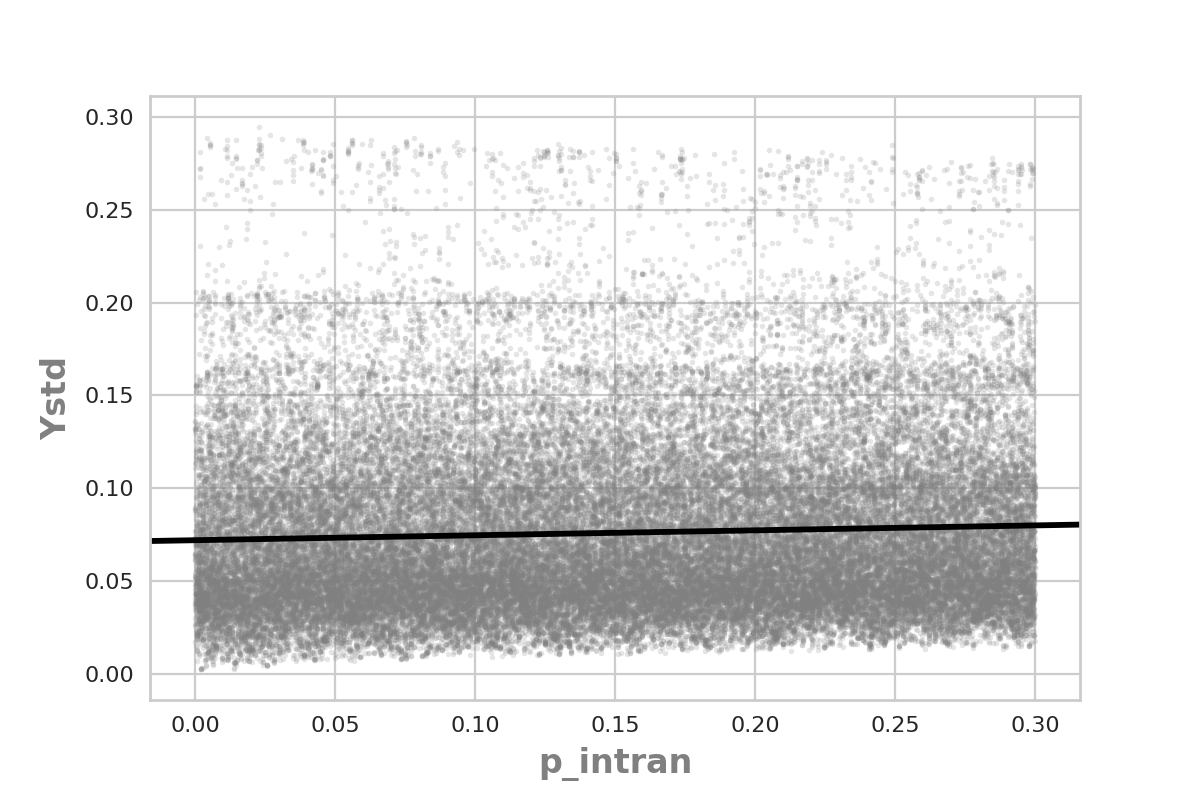
\includegraphics[width=\textwidth]{ims/mutoregressions/regressionmutatingop_intran.png}
    \end{subfigure}
    \caption{Gráfico de dispersão para 70.000 parametrizações.}
    \label{fig:scatter1}
    \source{ Elaborada pelo autor.}
\end{figure}

O parâmetro \(\rho\), o ruído, por sua vez, tem uma relação positiva com a
dispersão do sistema. Interessante notar, contudo, que o tamanho da população
parece não ter relação com o desvio padrão dos pontos ideais da população.

A intensidade dos parâmetros na variância da medida do sistema (Ystd) fica mais
claro na Figura \ref{fig:sobol1}:

\begin{figure}[H]
  \centering
  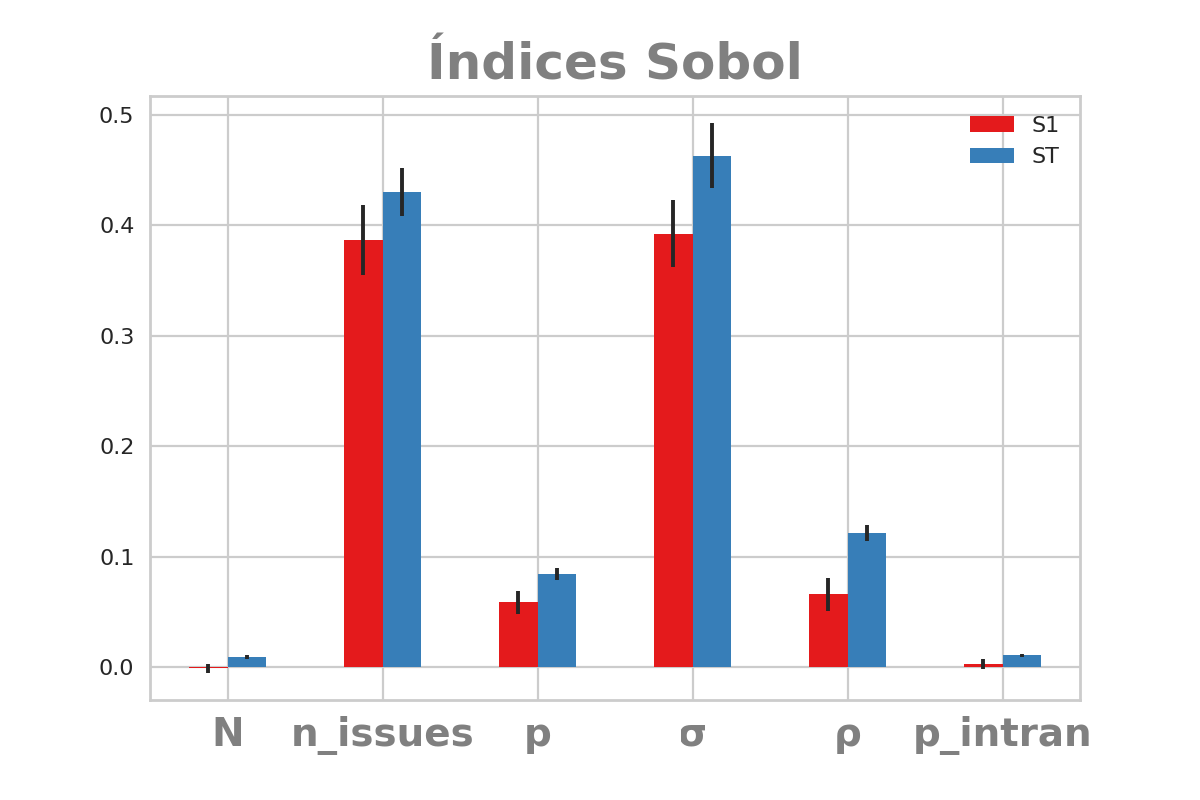
\includegraphics{ims/barplotmuto5k.png}
  \caption{Índices de Sobol de sensibilidade}
  \source{ Elaborada pelo autor.}
  \label{fig:sobol1}
\end{figure}

Como mostra a Figura \ref{fig:sobol1} o parâmetro \(N\) não tem impacto sobre a
variância de \(Ystd\), de forma que podemos tratá-lo como uma constante para
análise subsequentes. A figura mostra que a maior parte da variância na
dispersão dos pontos ideais pode ser explicada pelos parâmetros \(\sigma\), com S1\(
= 0.4621\) e ST \(= 0.5761\), e \(\text{n\_issues}\) e \(\rho\), que juntos tem um
S1\(= 0.32\). As somas dos S1 e ST são iguais a \(0.847\) e \(1.202\)
respectivamente, o que implica numa contribuição de \(0.3552\), que podemos
considerar grande, de efeitos interativos. Desses efeitos de interação entre
parâmetros 0.227 são devido a interações maiores do que de segunda ordem. Dentre
as de segunda ordem a maior interação é entre os parâmetros \(\sigma\) e \(\rho\).
Ademais, os coeficientes de erro são pequenos\footnote{Para os valores precisos
  ver as tabelas dos coeficientes S1, S2 e ST no Apêndice C.} tendo em vista que
a análise foi feita a partir de uma amostra grande, 70.000 parametrizações,
selecionadas por meio do método de Saltelli.

Um resultado contra-intuitivo é o baixo valor de impacto do parâmetro
\(p\_intran\). A comparação entre as figuras \ref{fig:tseries1} e
\ref{fig:tseries2} sugere que esse resultado seja um artefato da medida Ystd.

\begin{figure}[H]
    \centering
    \begin{subfigure}[b]{0.49\textwidth}
      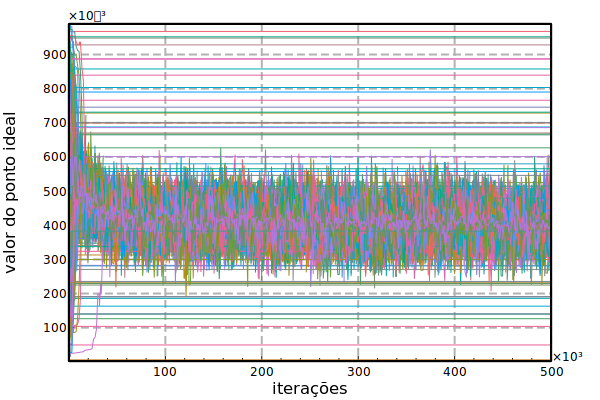
\includegraphics[width=\textwidth]{ims/timeseries3.png}
      \caption{\( \sigma = 0.1\) }
    \end{subfigure}
    \begin{subfigure}[b]{0.49\textwidth}
      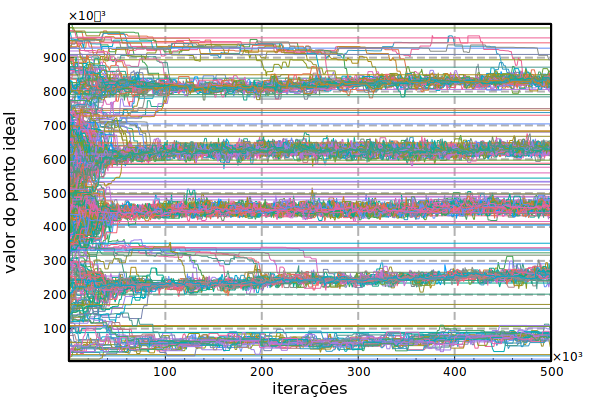
\includegraphics[width=\textwidth]{ims/timeseries4.png}
       \caption{\(\sigma = 0.02\) }
      \end{subfigure}
      \caption{Evolução dos pontos ideais dos agentes ao longo de duas realizações.
        Parametrização: \(p\_intran = 0.15, \text{ } N = 500,  \text{ }   p =
        0.9,  \text{ }  \rho = 1e-5,  \text{ }  n\_issues = 1 \)}
      \source{ Elaborada pelo autor.}
      \label{fig:tseries2}
    \end{figure}
    
    Enquanto na figura \ref{fig:tseries1} (a) o sistema converge para um único
    valor, na figura \ref{fig:tseries2} a população oscila no espaço ao redor
    desse valor. As figuras \ref{fig:tseries1} e \ref{fig:tseries2} (b) exibem
    uma diferença equivalente de comportamento. O parâmetro parece assim ter
    impacto sobre a dinâmica, particularmente sobre a
    cobertura\footnote{Definida da seção Metodologia de Análise}. Quais agentes
    são intransigentes é aleatório, mas como eles não mudam de opinião em um
    determinado tema é de se esperar que acabem por atrair os outros agentes
    para sua posição. Para testar a intuição de que os agentes intransigentes
    enviesam a dinâmica para a posição deles testamos a mesma parametrização que
    a figura \ref{fig:tseries2} (a), mas com os \(15\%\) intransigentes
    localizados entre os valores maiores que 0.8 ou menores que 0.2 no espectro
    ideológico. A figura \ref{fig:tseries3} demonstra que a atração para onde
    existem mais agentes intransigentes realmente ocorre\footnote{Com a figura
      \ref{fig:tseries3} replicamos o comportamento do modelo de
      \citeonline{deffuant2002can}.}.

      \begin{figure}[H]
    \centering
    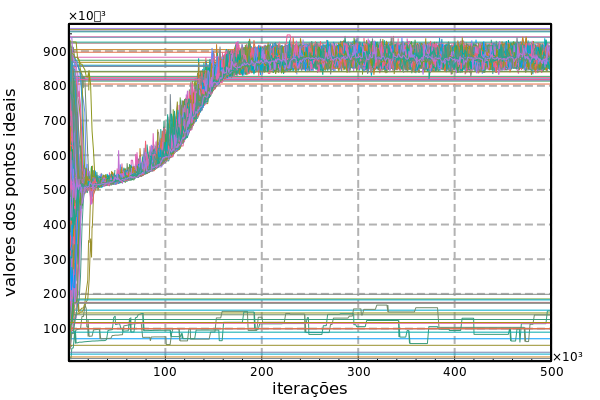
\includegraphics[scale=0.7]{ims/sigma01extremes.png}
    \caption{ Evolução dos pontos ideais dos agentes sob efeito de
      intransigentes nos extremos. Parametrização: \( \sigma = 0.1, \text{ }
      p\_intran = 0.15, \text{ } N = 500, \text{ } p = 0.9, \text{ } \rho = 1e-5,
      \text{ } n\_issues = 1 \)}
    \source{ Elaborada pelo autor.}
    \label{fig:tseries3}
  \end{figure}

  Um caso interessante a ser considerado é quando existem agentes intransigentes
  na população, mas a intransigência deles não é absoluta, o valor de \(\sigma\) não
  é tão baixo. Testamos o efeito de intransigentes com \(\sigma = 0.01\) tanto
  distribuídos ao longo do espaço ideológico quanto somente nos extremos. No
  caso de agentes intransigentes extremistas temos um comportamento semelhante
  ao da figura \ref{fig:tseries3}, a convergência de grande parte da população
  para um dos extremos. O que difere é que o \textit{cluster} maior agora
  converge para um único valor, enquanto com intransigentes absolutos ele oscila
  dentro de um dos extremos.

    \begin{figure}[H]
    \centering
    \begin{subfigure}[b]{0.49\textwidth}
      \includegraphics[width=\textwidth]{ims/n1-sigma1.png}
      \caption{Intransigentes ideologicamente distribuídos.}
    \end{subfigure}
    \begin{subfigure}[b]{0.49\textwidth}
      \includegraphics[width=\textwidth]{ims/n1-sigma1-extremes.png}
       \caption{Itransigentes localizados nos extremos.}
     \end{subfigure}

     \caption{ Intransigentes com \(\sigma = 0.01\). Parametrização global: \( \sigma =
       0.1, \text{ } p\_intran = 0.15, \text{ } N = 500, \text{ } p = 0.9,
       \text{ } \rho = 1e-5, \text{ } n\_issues = 1 \)}
    \source{ Elaborada pelo autor.}
    \label{fig:newintrans}
     \end{figure}
  
     Curiosamente, quando os agentes intransigentes estão localizados ao longo
     do espaço e não são absolutamente intransigentes temos um comportamento
     totalmente distinto. Ao invés de haver a manutenção da tendência central
     dada pelo \(\sigma\) global igual a 0.1, como demonstrado na figura
     \ref{fig:tseries2}, ocorre uma convergência da maioria da população para um
     dos extremos, sem precisarmos estabelecer previamente que todos os
     intransigentes vão estar nos extremos. Nesse caso, da figura
     \ref{fig:newintrans} (a), o \textit{cluster maior} vai ``varrendo'' um dos
     lados do espaço sendo atraído pelos  intransigentes desse lado até um dos extremos.
     Esse comportamento sistêmico, contudo, depende tanto do tamanho da
     população quanto do número de iterações. Como demonstrado na figura
     \ref{fig:newintrans2} quanto menor o tamanho da população menos iterações
     são necessárias para que a maioria da população seja atraída para um dos
     extremos.
  \begin{figure}[H]
    \centering
    \begin{subfigure}[b]{0.49\textwidth}
      \includegraphics[width=\textwidth]{ims/sigma01_pop200.png}
      \caption{N = 200}
    \end{subfigure}
    \begin{subfigure}[b]{0.49\textwidth}
      \includegraphics[width=\textwidth]{ims/sigma01_pop700.png}
       \caption{N = 700}
     \end{subfigure}

         \begin{subfigure}[b]{0.49\textwidth}
      \includegraphics[width=\textwidth]{ims/sigma01_pop1000.png}
       \caption{N = 1000}
     \end{subfigure}
         \begin{subfigure}[b]{0.49\textwidth}
      \includegraphics[width=\textwidth]{ims/sigma01_pop1200.png}
       \caption{N = 1200}
     \end{subfigure}

     \caption{ Intransigentes com \(\sigma = 0.01\). Parametrização global: \( \sigma =
       0.1, \text{ } p\_intran = 0.15, \text{ } p = 0.9,
       \text{ } \rho = 1e-5, \text{ } n\_issues = 1 \)}
    \source{ Elaborada pelo autor.}
    \label{fig:newintrans2}
     \end{figure}
  

  
    Como nem o desvio padrão nem o número de pontos ideais finais,
    como discutido anteriormente, nos dão medidas quantitativas desses impactos
    passamos a uma análise gráfica de certas combinações de parâmetros típicas.
    Os gráficos de dispersão nos indicam\footnote{Regressões polinomiais de
      terceira ordem foram usadas para auxiliar essa análise. Estão no
      Apêndice D.} possíveis restrições aos limiares dos parâmetros.

    Dado o pequeno impacto de \(N\) e \(p\) vamos mantê-los constantes, com
    valores de 500 e 0.9 respectivamente. Uma conjunto de parametrizações não
    abarcado pela análise de sensibilidade global é quando \(p\_intran = 0.0, \rho \approx
    0 \). Nesse caso, se tivermos como base \(N = 500\), é possível usar o
    número de pontos ideais finais como medida do sistema, de forma que podemos
    analisar o papel tanto de \(\sigma\) quanto de \(n\_issues\) num sistema sem
    ruído e sem intransigentes. Testamos 100 realizações para cada
    parametrização e representamos o resultado, o número de pontos ideais finais
    após 1.000.000 de iterações, por meio de diagramas de caixa.
    
  \begin{figure}[H]
    \centering
    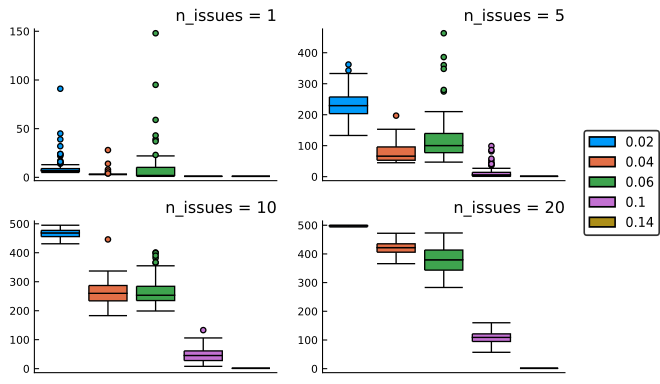
\includegraphics[scale=0.7]{ims/boxes4.png}
    \caption{Número de pontos ideais finais para diferentes valores de \(\sigma\).
      Parametrização: \(\rho =1e-5, p\_intran = 0.0, p = 0.9, N =500\)}
    \source{Elaborada pelo autor.}
    \label{fig:box4}
  \end{figure}
  
  Como mostra a figura \ref{fig:box4} quanto maior o valor de \(\sigma\) menor a
  cobertura da configuração final. Um resultado que aparenta ser contrário ao da
  análise anterior é que quanto maior o número de questões \textit{maior} a
  cobertura final, enquanto que a análise anterior demonstrou uma relação
  negativa entre número de questões e dispersão. Isso só é verdade pelo fato dos
  parâmetros \(\rho\) e \(p\_intran\) serem nulos, ou aproximadamente nulos. Nesse
  caso aumentar o número de questões faz com que sejam necessárias mais
  interações entre os agentes para que eles se aproximem ideologicamente, já que
  pelo procedimento da simulação eles só atualizam uma opinião por vez. Isso faz
  com que aumentar o número de questões contribua para uma maior dispersão e
  cobertura de posicionamento ideológicos.
  
  Contudo, a partir do momento que a proporção de agentes intransigentes e o
  ruído são não-nulos o número de questões passa a ter o efeito contrário. Como
  demonstrado na figura \ref{fig:tseries4} quando \(n\_issues = 1\) o sistema
  passa a ter sua configuração facilmente controlada por aqueles parâmetros.
  Como só há uma única questão os agentes quando sofrem o efeito do ruído
  passeiam pelo espectro todo. Já quando interagem com agentes intransigentes
  tem seu ponto ideal atraído bem mais em direção a opinião deles, em
  contraposição ao caso em que seu ponto ideal é derivado de várias opiniões,
  pois mesmo que o agente mude, aleatoriamente ou sob o efeito da interação com
  um agente intransigentes, \textit{uma} de suas opiniões o ponto ideal é
  estabilizado pelo posicionamento dele em outras questões. O número de questões
  serve então para controlar o efeito dos agentes intransigentes e do ruído, e
  tornar mais robusto o efeito de concentração ditado por \(\sigma\), o parâmetro de
  maior impacto.


    
\begin{figure}[H]
    \centering
    \begin{subfigure}[b]{0.49\textwidth}
      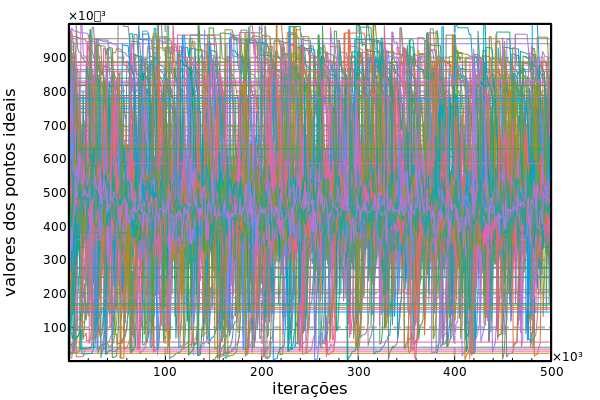
\includegraphics[width=\textwidth]{ims/n1-sigma01.png}
      \caption{\( n\_issues = 1,  \sigma = 0.1\) }
    \end{subfigure}
    \begin{subfigure}[b]{0.49\textwidth}
      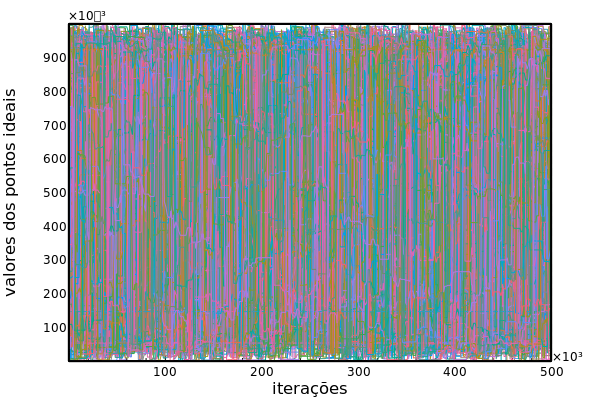
\includegraphics[width=\textwidth]{ims/n1-sigma002.png}
       \caption{\(n\_issues = 1, \sigma = 0.02\) }
     \end{subfigure}

     \begin{subfigure}[b]{0.49\textwidth}
       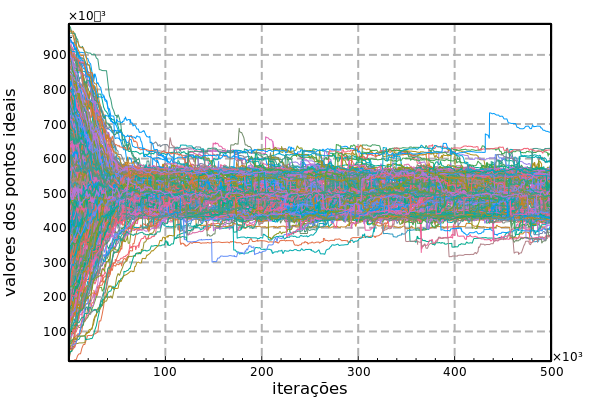
\includegraphics[width=\textwidth]{ims/n7-sigma01.png}
       \caption{\(n\_issues = 7, \sigma = 0.1\)}
     \end{subfigure}
     \begin{subfigure}[b]{0.49\textwidth}
       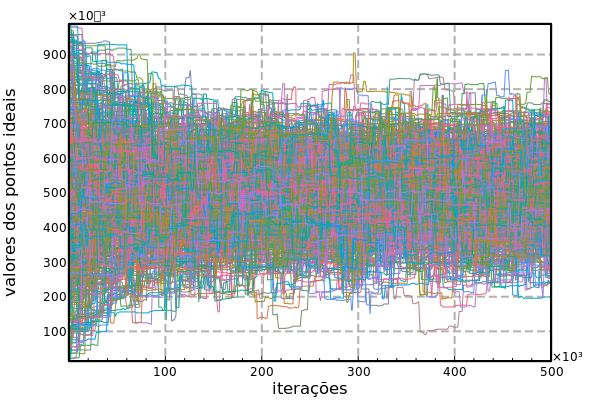
\includegraphics[width=\textwidth]{ims/n7-sigma002.png}
       \caption{\(n\_issues = 7, \sigma = 0.02\)}
     \end{subfigure}
      \caption{Evolução dos pontos ideais quando há ruído e agentes intransigentes.
        Parametrização: \(p\_intran = 0.15, \text{ } N = 500,  \text{ }   p =
        0.9,  \text{ }  \rho = 0.05\)}
      \source{ Elaborada pelo autor.}
      \label{fig:tseries4}
    \end{figure}


\todo[inline,color = yellow!10]{Fazer as considerações indicadas por André.}

    
%%% Local  Variables:
%%% mode: latex
%%% TeX-master: "master"
%%% End:
